\chapter{M/M/1 simulation}


\section{NS-3}

NS-3 is a discrete-event network simulator, targeted primarily for research and educational use.
NS3 is used to simulate modern network systems with real time scheduler many used for academic and research purposes.


\section{Model implementation}

We implemented M/M/1 queuing model in ns3 which can take inputs like lambda referring to arrival rate, mu referring to service rate, initialpackets referring to number of packets in queue initially, numpackets referring to number of packets to en-queue, queue limit referring to size of the queue. The packets are scheduled to be en-queued according to the arrival rate, and the packets are dequeued according to the service rate.\\
We log all the activity happening in the queue system and collect traces and store them in a .dat file.

\section{Simulation results}

We study the idle time of the queue, mean queue length, and average packet delay, while varying the arrival rate from $\lambda = $ 1 to 9 keeping service rate constant at $\mu=10$. We send 1,00,000 packets and keep queue limit a relatively large value to avoid packet drops

We plot the results below,
\begin{figure}[H]
    \centering
    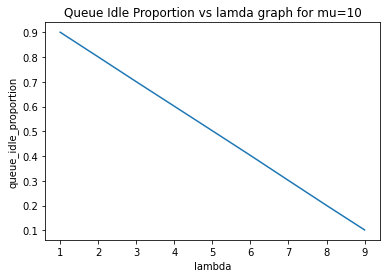
\includegraphics{idle_vs_lamda.png}
    \caption{Idle time of queue}
    \label{fig:idle}
\end{figure}
Increasing lambda linearly decrease the idle proportion of the queue linearly following the formula $P(idle)=1-\rho$

\begin{figure}[H]
    \centering
    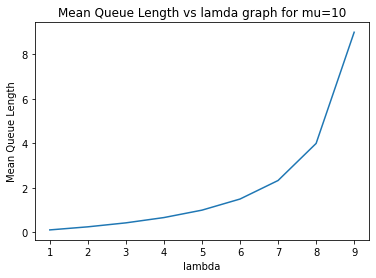
\includegraphics{length_vs_lamda.png}
    \caption{Avg length of queue}
    \label{fig:lenvslambda}
\end{figure}

Length of the system in steady state is consistent with the given by the formula, $L_s=\frac{\rho}{1-\rho}$
\begin{figure}[H]
    \centering
    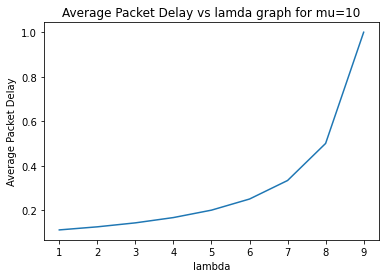
\includegraphics{packet_delay_lamda.png}
    \caption{Packet delay}
    \label{fig:delay}
\end{figure}

Mean Delay of packets is consistent with the formula $W_s = L_s/\lambda=\frac{1}{\mu-\lambda}$
\\

Next we experiment with the buffer overflow times for sending 1,00,000 packets in the M/M/1 queue starting with no packets initially in the queue with the buffer queue size of 100 packets. We fix µ = 10 and run the simulation varying lambda values as follows $\lambda$ = 9.5, 9.7, and 9.9. We measure how long it takes for the queue to overflow.

\begin{figure}[H]
    \centering
    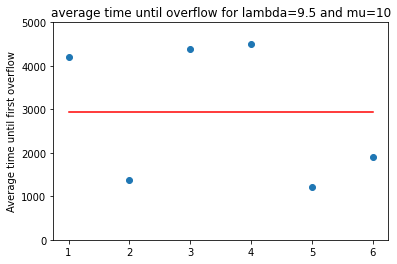
\includegraphics{95.png}
    \caption{Overflow times for lambda=9.5}
    \label{fig:95}
\end{figure}
The individual points represent the times at which the queue overflowed for the first time for different simulation runs with $\lambda=9.5$.
The horizontal line represents the average of the overflow times of these simulations
\begin{figure}[H]
    \centering
    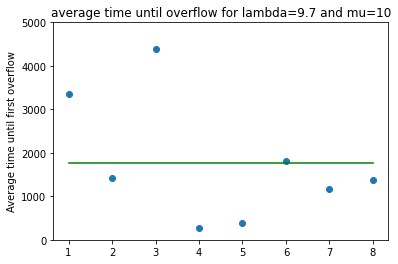
\includegraphics{97.png}
    \caption{Overflow times for lambda=9.7}
    \label{fig:97}
\end{figure}
The individual points represent the times at which the queue overflowed for the first time for different simulation runs with $\lambda=9.7$.
The horizontal line represents the average of the overflow times of these simulations
\begin{figure}[H]
    \centering
    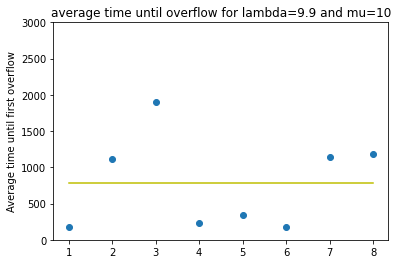
\includegraphics{99.png}
    \caption{Overflow times for lambda=9.9}
    \label{fig:99}
\end{figure}
The individual points represent the times at which the queue overflowed for the first time for different simulation runs with $\lambda=9.9$.
The horizontal line represents the average of the overflow times of these simulations


We can see that the average time until first overflow decreases with lambda value coming close to mu, this behaviour is expected as the increased arrival rate congest the queue faster and probability of a packet dropped from the queue increase at lower times.
